\restylefloat{table,figure}
\pagestyle{fancy}
\cfoot{\thepage}
\renewcommand{\footrulewidth}{0.25pt}


 
\section{Clustering}
\subsection{Introduzione}

L'analisi di cluster è usata per risolvere moltissimi problemi pratici. In particolare l'\textbf{analisi di cluster tratta due diversi scopi generali:}

\begin{itemize}
	\item \textbf{Comprensione}: Le classi, o gruppi di oggetti che condividono caretteristiche, giocano un ruolo importante nella comprensione del mondo. Questo succede in biologia, in informatica e in economia.
	\item \textbf{Utilità}: Capacità di risassumere determinate carateristiche di un oggetto con le caratteristiche del cluster a cui appartiene. L'obiettivo è \textit{trovare i prototitpi con le proprietà più rappresentative dei cluster}.
\end{itemize}

Possiamo dare ora una definizione un po' più completa di analisi di clustering.
\begin{defn}
	La \textbf{cluster analysis} raggruppa i dati basandosi sulle informazioni trovate nei dati che descrivono gli oggetti e le loro relazioni.
\end{defn}

Gli obiettivi sono ora semplici da ridefinire:
\begin{itemize}
	\item Gli oggetti all'interno di un gruppo devono essere simili gli uni con gli altri, allo stesso tempo diversi (o incorrelati) con gli oggetti di altri gruppi.
	\item La più grande \textit{similarità} entro un gruppo deve corrispondere ad una grande \textit{differenza} tra i gruppi. 
\end{itemize}

\underline{Problema}: Come faccio a stabilire quando  e quanto degli oggetti sono simili? Non vi è un metodo per capirlo, tendenzialmente si utilizza una soluzione intermedia rispetto alle altre. 

La definizione di cluster è \textbf{intrinsicamente imprecisa},una migliore definizione dipende infatti dalla natura dei dati e dai risultati desiderati. 

\subsubsection{Tipi di clustering}

Formare un insieme di cluster è chiamato in gergo tecnico \textit{clustering.} Ci sono diversi tipi di analisi di clustering.

\begin{itemize}
	\item Partitional vs Hierarchical
	\item Exclusive vs  Overlapping vs Fuzzy
	\item Complete vs Partial.
\end{itemize}

Diamo ora una rapida definizione di tutte:

\begin{defn}
	Un clustering si dice \textbf{partizionale} se vi è una divisione del dataset in insiemi non sovrapposti tali che un elemento appartiene ad un solo insieme.
\end{defn}

\begin{defn}
	Un clustering si dice \textbf{gerarchico} se ogni cluster può essere a sua volta suddiviso in sotto cluster, in questo caso il clustering è un insieme di cluster che sono organizzati come un albero.
\end{defn}

\begin{defn}
	Un clustering si dice \textbf{esclusivo} se ogni oggetto è assegnato ad un singolo cluster.
\end{defn}

\begin{defn}
	Un clustering si dice \textbf{sovrapponibile} se ogni oggetto può essere assegnato a più di un cluster.
\end{defn}

\begin{defn}
	Un clustering si dice \textbf{fuzzy} se ogni oggetto può essere assegnato a più di un cluster contemporaneamente con un valore che tiene conto del peso che ha l'oggetto rispetto all'appartenenza ad un singolo cluster, la somma dei pesi deve essere necessariamente 1.
\end{defn}
\begin{figure}[H]
	\centering
	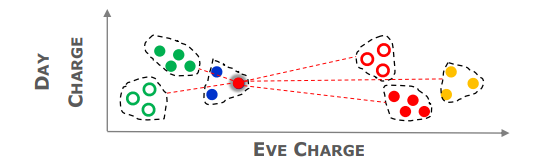
\includegraphics[height=0.3 \linewidth]{clustering/pict/fuzzy.png}
	\caption{Custering con modello fuzzy}
\end{figure}
\begin{defn}
	Un clustering si dice \textbf{completo} se ogni oggetto è assegnato ad un cluster (non ci sono oggetti liberi).
\end{defn}

\begin{defn}
	Un clustering si dice \textbf{parziale} se esiste almeno un oggetto che non è assegnato a nessun cluster, si usa perché potrebbero esserci degli outlier ed inserirli all'interno di un cluster potrebbe peggiorare in modo significativo la rappresentazione di un cluster.
\end{defn}

\subsubsection{Differenti nozioni di cluster}
I cluster naturali sono cluster che si dicano esistano per davvero anche se questo  è molto difficile che ciò accada. Per visualizzare le differenze tra i tipi diversi di dati sfruttiamo dati come punti a due dimensioni.
\begin{itemize}
	\item \textbf{Well separated Cluster:} dato un cluster, ogni oggetto è più vicino ad ogni oggetto del cluster a cui appartiene piuttosto che a qualsiasi altro oggetto di ogni altro cluster. Un cluster così ben formato permette di avere separazioni molto nette, questo tipo di cosa succede però molto raramente in realtà.
	\item \textbf{Prototpe-based cluster} dato un cluster, ogni oggetto di quel cluster è più vicino al prototipo che definisce il cluster rispetto ad ogni prototipo di un altro cluster. Il prototipo \`e solitamente il \textit{centroide} del cluster. Il \textit{prototipo} di un cluster corrisponde all'individuo meglio rappresentato dal cluster (può essere anche fittizio). Cluster fatti in questo modo tendon ad essere globulari.
	\item \textbf{Density-based cluster} un cluster è una regione densa di oggetti che sono circostritti da una regione di bassa densità. Questi sono usati quando i cluster sono irregolari o intermittenti oppure quando c'è una grande presenza di rumore o di outlier.
	\item \textbf{Graph-based cluster} se i dati sono rappresentati da grafi, i nodi rappresentano  oggetti e i collegamenti connettono gli oggettti. Allora ogni cluster è una componente connessa. La connessione può anche essere pesata e scelta in base ad una certa soglia. 
	Questi cluster sono molto utilizzati in quanto c'è un sacco di ricerca già fatta.
\end{itemize}

\subsubsection{Componenti di un'analisi di clustering}

Per prima cosa  avviene la \textit{feature selection} che assicura la trattenuta degli attributi del dataset degni di significato. Successivamente avviene la fase di  \textit{feature extraction} che serve a produrre feature che potrebbero andare meglio per scoprire la struttura dei dati, questa pratica potrebbe tuttavia generare features di difficile comprensione.
Le feature ideali 

\textbf{ARRIVATO QUIIIIII}
 Applicare un algoritmo di clustering, per poterlo fare devo specificare una misura di affinit\`a. Successivamente bisogna capire come impostare l'ottimizzazione di una misura di merito scelta. Dopo tutto ci\`o bisogna ricriticare tutto ci\`o che si \`e fatto e valutare il funzionamento e le eventuali performance, entrare nel merito e valutare se i gruppi siano sensati. Si tratta di investigazione sul clustering. Successivamente si cerca un'interpretazione dei risultati chiedendo all'esperto di dominio cosa ne pensa. Saranno i cluster non compretamente palesi all'esperto i pi\`u interessanti da valutare. 



\subsection{Lezione 11 - Proximity}

La proximity \`e uno strumento fondamentale per valutare il funzionamento di un algoritmo di clustering. 

La cluster analysis affonda le sue radici in cosa sia \textbf{simile} e cosa sia \textbf{dissimile}. La similarit\`a \`e un conetto relativo, nel senso che posso considerare uno smartphone e un telefono simili se li considero come strumenti di comunicazione per\`o non per quanto riguarda la forma.

La \textbf{similarit\`a} \`e un valore alto per paia di oggetti che si assomigliano e solitamente si usa un valore compreso tra 0 e 1. 

La \textbf{dissimilarit\`a} \`e una misura numerica di gradi per i quai due oggetti sono differenti. In generale si cerca di ricodurla in un intervallo $[0,1]$ per\`o anche di $[0,\inf]$.

La \textbf{prossimit\`a} ulilizza riferimenti a similarit\`a e dissimilarit\`a.

\begin{figure}[h!]
	\centering
	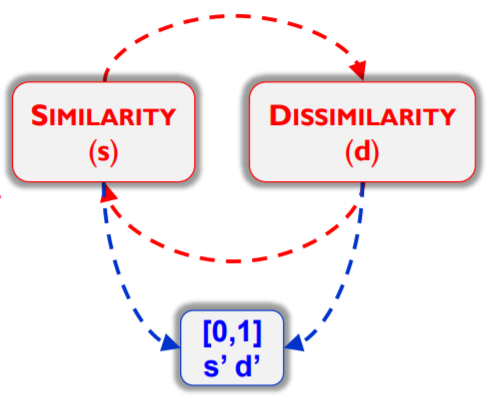
\includegraphics[height=0.45 \linewidth]{clustering/pict/simil_diss.png}
	\caption{vantaggi e svantaggi tra tecniche uni-variate e multi-variate}
\end{figure}

Se voglio trasformare una misura di similarit\`a in $[0,\inf]$ allora ho bisogno di una trasformazione \textbf{non lineare} e la relazione tra i valori non avr\`a la stessa scala. Verranno compressi dei valori in valori distorti. (\textit{in alcuni casi distorcere i valori \`e quello che desidero}). 

La trasformazione tra similarit\`a e dissimilarit\`a e sostanzialmente lineare, bisogna scegliere un metodo per metterli in relazione. 

Comunque, la \textbf{prossimit\`a} tra due record \`e una funzione di prossimit\`a compresa tra i corrispondenti attributi dei due record.

Per quanto riguarda gli attributi binari la dissimilarit\`a esclude la similarit\`a con valori 0 e 1. 

Se ho attributi nominali ordinali assegno un valore intero agli stessi in base alla scala utilizzata e calcolo la dissimilarit\`a come rapporto tra la differenza dei due record e la scala totale di valori di utilizzo. Naturalmente va notato che sto utilizzando una scala linerare! (forte assunzione)

Qualsiasi scala di valori si andr\`a a scegliere si porter\`a dietro delle assunzioni.

\subsection{Misure della distanza}
Le distanze sono dissimilarit\`a con certe propriet\`a, quando tutti gli attributi sono numerici.

\begin{figure}[h!]
	\centering
	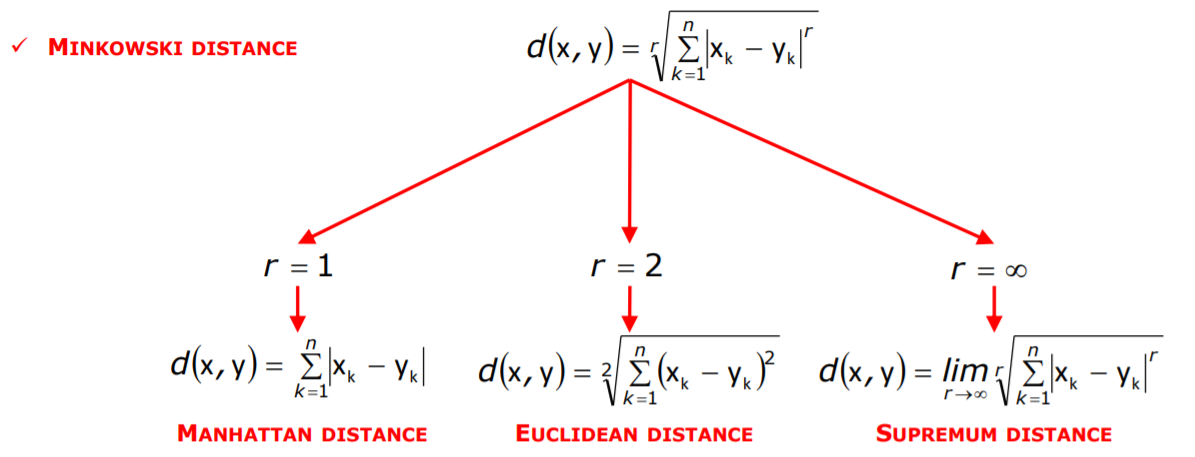
\includegraphics[height=0.4 \linewidth]{clustering/pict/distanze_minkowski.png}
	\caption{vantaggi e svantaggi tra tecniche uni-variate e multi-variate}
\end{figure}

La misura deve essere
\begin{itemize}
	\item non negativa
	\item simmetrica
	\item disuguaglianza triangolare
\end{itemize}

La similarit\`a solitamente non rispetta la disuguaglianza triangolare ma \`e simmetrica e non negativa. 

\textbf{Misure di coefficienti}

Simple matching coefficient: \[ SMC(x,y) = \frac{\#maching attriutes}{\#attributes} \]

Questa misura ci piace quando gli 0 e gli 1 sono gli stessi. Si dice che gli 0 sono molto meno nobili degli 1. \`E una misura equilibrata.

Jaccard Coefficient \[ J(x,y) = \frac{\#of matching presences}{\# attibutes except 00 matches}\]

Questa misura distorta rispetto gli 1 mi permette per\`o di focalizzare la mia attenzione sugli 1. 

Una versione di questo indice \`e la Extended Jaccard Coefficient, viene utilizzato nell'analisi di testo in linguaggio naturale (Es. post su twitter) analizza vettori di attributi.

\[ EJ(x,y) = \frac{x \cdot y}{||x||^2 + ||y||^2 - x \cdot y}\]


\textbf{Similarit\`a al coseno}, utilizzata quando gli attributi hanno natura numerica (utilizzata in information retrival).

\textbf{Correlazione} quella di Pearson ma non legato a variabili aleatorie, bensì quelle con i vettori. 

Problemi:
\begin{itemize}
	\item come trattare attibuti su scale di ampiezza diverse e correlati
	\item come calcolare la prossimit'` a tra record composti da attributi di tipo diverso
	\item come trattare la prossimit\`a quando assegnavo una diversa rilevanza a diversi attributi, non tutti contribuiscono allo stesso modo
\end{itemize}

nel primo caso bisogna normalizzare i valori in modo che rispettino la stessa scala e poi applicarci misure di distanza come la euclidea, quando invece tutti gli attributi sono correlati e la distribuzione approssimata dalla gaussiana allora uso la distanza di Mahalanobis

nel terzo caso la similarit\`a diventa:

formula con i pesi della similarit\`a 

Indicazioni generali:

\begin{itemize}
	\item dati densi e continui: distanza come quella euclidea buona rappresentazione
	\item dati sparsi, binari asimmetrici: misuri della distanza che ignorano i match 00 come cosine, Jaccard e Extended Jaccard
\end{itemize}

\subsection{Clustering Algorithms}

\textbf{Prototype-Based Custering} un cluster \`e un sottoinsieme di oggetti come vicini (similarit\`a o dissimilarit\`a) rispetto ad un oggetto prototipo. 

\begin{figure}[h!]
	\centering
	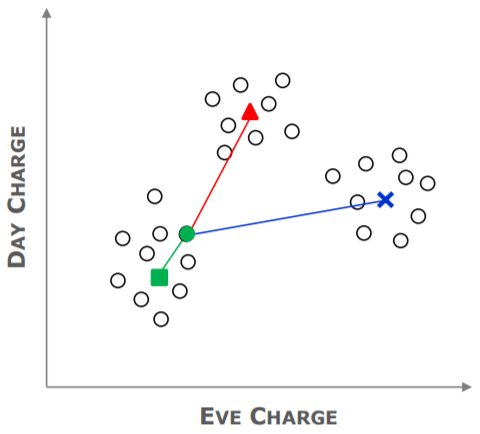
\includegraphics[height=0.4 \linewidth]{clustering/pict/prototype_cluster.png}
	\caption{esempio di prototype-based clustering}
\end{figure}

il quadratino, triangolino e x sono i prototipi centroidi dei cluster. Mi focalizzo su un'osservazione e essa viene assegnata al cluster del centroide prototipo pi\`u vicino.

Caratteristiche:
\begin{itemize}
	\item oggetti appartengono ad un unico cluster
	\item oggetti sono condizione di appartenere a pi\`u di un gruppo
	\item un cluster \`e modellato con una interpretazione probabilistica
	\item i cluster sono vicolati ad avere relazioni fisse (vicinato)
\end{itemize}

\subsection{K-medie}
Il prototipo in questo caso prende il nome di \textbf{centroide}, di solito \`e indentificato dal vettore media dei valori degli attributi delle osservazioni di quel determinato cluster (quindi dei record). Solitamente applicato a oggetti in uno spazio continuo n-dimensionale.

Bisogna comunque dichiarare il \underline{numero di cluster} da identificare (K cluster) e fa la differenza questo parametro!! 

\subsubsection{Algoritmo}
\begin{enumerate}
	\item Selezione K oggetti come centrodi
	\item \textbf{Reapeat} (ciclo)
	\item Da K cluster, assegnamo ogni record al centroide pi\`u vicino
	\item Ricalcola il centroide di ogni cluster
	\item \textbf{Until} i centroidi non cambiano
\end{enumerate}

\section{Lezione 12 - Clustering Algorithm}

\textbf{K-mean}: vi sono diverse misure di sitanza che popssono essere applciate [errata corrige: massimizzare la somma di coseno (slide 3 part II)]

Problemi sono:
\begin{itemize}
	\item la scelta dei iniziale centroidi \`e fondamentale e influenza in modo pesante le performance dell'algoritmo in generale. Vi sono alternative quali il clustering gerarchico.
	\item punti a favore del K-medie \`e che occupa il minimo spazio ed \`e un algoritmo abbastanza rapido in quanto \`e lineare per il numero di istanze considerate. 
	\item pu\`o accadere che un cluster sia vuoto per scelta sbagliata di centroidi iniziale (magari randomica).
	\item problema di Outlier: crea grossi problemi quando calcolo la media delle osservazioni di un cluster (\`e per\`o efficiente nella ricerca di outlier in quanto li indentificher\`a come sigleton)
	
\end{itemize}

Limiti sono:
\begin{itemize}
	\item difficolt\`a a ricercare cluster di non forma sferica
	\item difficolt\`a a trovare cluster con dimensioni diverse
	\item difficolt\`a a indentificare cluster di diversa densit\`a (vicinanza dei punti)
\end{itemize}

Per ovviare ad alcuni di questi problemi vi sono tecniche per clusterizzare in cluster pi\`u numerosi ed alla fine unire secondo degli algoritmi specifici nel numero di cluster richiesto, es minimizzazione delle distanze dei centroidi. 

Quindi K-medie \`e:
\begin{itemize}
	\item semplice e si applica a tanti tipi di dati
	\item \`e abbastanza efficiente anche se vengono effettuate pi\`u applicazioni successive dello stesso
	\item vi sono varianti pi\`u efficienti e meno problmatiche (es. bisecting k-means)
	\item non adatto a tutti i tipi di dat e non pu\`o gstire cluster non sferici, con size e densit\`a diverse
	\item problemi con dati outliers
	\item \`e strettamente legato al concetto di centroide. Vi sono delle varianti che utilizzano il \underline{medoide} ed \`e pi\`u efficiente
	
	
\end{itemize}
NB: pi\`u cluster vengono utilizzati pi\`u aumenta la complessit\`a computazionale.


\subsection{Fuzzy C-means}
Se gli elementi sono distribuiti in gruppi ben separati il clustering \`e semplice, i problemi nascono dove le istanze sono molto vicine. Inoltre consideriamo il fatto di osservazione sulla frontiera delle distanze dei cluster. 

Per ovviare al problema ogni osservazione viene considerata come appartenente ad ogni cluster ma con una misura diversa per ognuno! (es. utilizzando la misura della media)

$w_{ij}$ \`e il \textbf{peso} con cui l'$i$-esimo oggetto appartiee al $j$-esimo cluster.

La \textbf{pseudo-partizione Fuzzy} \`e definita assegnando prima l'isieme di tutti i pesi $w_{ij}$ con $w_{ij} \geq 0$ ed essi devono essere verificati dai seguenti vincoli:

\[\sum_{j=1}^{K} w_{ij} = 1\] con $i = 1, ..., m$

\[ 0 < \sum_{i=1}^{m}w_{ij} < m\] con $j = 1, ..., K$

Ogni oggetto deve essere assegnato ad un certo grado a tutti i cluseter. Non sono permessi cluster vuoti e ogni oggetto pu\`o essere assegnato esclusivamente ad un singolo cluster.

Il Fuzzy C-means produce cluseter che danno un'indicazione del grado in cui ogni oggetto appartiene ad ogni cluster, ha gli stessi punti di forza e debolezza del K-means ma pi\`u pesante computazionalmente.

\subsection{Modelli a mistura}
In questi modelli vediamo le osservazioni da una mistura di diverse distribuzioni di problabilit\`a. In sostanza possiamo vedere le misture come distribuite secondo delle normali con uguale varianza ma medie diverse (curve di livello) [propriet\`a rilassabile]. 

Supponiamo spazio di 3 componenti, processo di generazione:
\begin{enumerate}
	\item Seleziono uno delle 3 componenti
	\item Estraggo un campione dalla componente selezionata
	\item ripeto 1 e 2 m volte per ottenere il dataset
\end{enumerate} 

\[ p(\bar{x}|\Theta) = \sum_{j=1}^{K} w_j p(\bar{x}|\theta_j)\] probabilit\`a dell'oggetto x dove $w_j$ probabilit\`a della j-esima componente, $p(\bar{x}|\theta_j)$ probabilit\`a di estrarre x dalla j-esima component, $\theta_j$ parametri associati a j.

Il processo sostanzialmente \`e quello di partire dai dati e ridurrli nelle misture significative. (simile a come avviene la nostra capacit\`a di isolare il rumore uditivo). Vi \`e un algoritmo utilizzato per la risoluzione che \`e l'\textbf{Expectation Maximization}. Si tratta di una classe di algoritmi che sono diversi in base alla loro applicazione. 

Svantaggi:
\begin{itemize}
	\item Apprendimento \`e lento
	\item non \`e pratico per i modelli con un gran numero di componenti
	\item non funziona bene quanto i cluster conengono  poche osservazioni
	\item non funziona bene quando gli oggetti sono co-lineari
\end{itemize}

\begin{itemize}
	\item pi\`u generico di k-means e fuzzy c-means perch\`e usa distribuzioni di vario tipo
	\item disciplina l'approccio di eliminazione di complessit\`a
\end{itemize}


\subsection{Mappe di Kohonen o SOMs}
Una struttura feedforward per algoritmi di clustering. Detta anche mappa atorganizzante. Vi \`e una mappatura dei neuroni che mappano in uno spazio bidimensionale. Non hanno una sola direzione ma sono bi-direzionali, possono spostare i pesi sia da input ad output che viceversa.

Ho uno spazio di input continuo e voglio mapparlo in uno spazio discreto di output. Vorrei che mappando un'osservazione in un neurone posso poi tornare indietro tramite un altro collegamento.

Vi \`e un'informazione topografica in tutto ci\`o. Ed \`e una cosa unica rispetto agli altri algoritmi di clustering considerati. Durante la fase di apprendimento sfruttiamo la topologia considerando ogni oggetto aggiornato al centroide pi\`u vicino secondo essa. Considerando un neurone assegnato ad una osservazione, allora anche i neuroni ad esso adiacenti (vicinato - definito in vari modi) dovrebbero risentirne di questo assegnamento, in questo modo vengono trainati i neuroni e i vicini degli stessi. 

Riassumendo:
\begin{enumerate}
	\item inizializzazione, seleziono i centroidi assocaiti a ciascun neurone
	\item competizione tra diversi neuroni per ottenere l'istanza. Ogni neurona fa un'offerta diversa per vincere quell'oggetto e la proposta \`e proporzionata in base a quanto un neurone (in base al suo centroide) si considera "vicino" all'istanza considerata, viene poi proclamato il vincitore e gli viene assegnata l'istanza (in base a una misura di performance)
	\item collaborazione una volta che un neurone vince distribuisce il suo vantaggi ai vicini (processo di premi-punizioni) aggiustando i centroidi
	\item aggiornamento del centroide del vincitore e dei vicini calcolandol attraverso l'istanza appena considerata
\end{enumerate} 

Punti di forza Interpretabilit\`a dei cluster 

Limiti:
\begin{itemize}
	\item bisogna scegliere un gran numero di parametri, funzione di vicinato ecc e varia molto nelle performance
	\item non sempre un raggruppamento identifica un singolo cluster naturale (solitamente dopo viene applcato un k-medie sui centroidi trovati)
	\item difficile paragonare i risultati
	\item la convergenza non \`e garantita, \`e un'euristica
\end{itemize}

\section{Lezione - Clustering Algorithm}

\subsection{Clustering Gerarchico}
\begin{itemize}
	\item \textbf{agglomerativo}: si parte da tutti gli oggetti come cluster individuali e ad ogni step unisce le coppie di cluster pi\`u vicine.
	\item \textbf{divisivo}: parte da un cluster unico e passo passo divide il cluster in soli cluster singleton di oggetti individuali rimanenti. Abbiamo bisogno di decidere quale cluster splittare ad ogni passo e come splittare
\end{itemize}

\textbf{Clustering gerarchico agglomerativo} sono i pi\`u comuni. La soluzione che si ottiene \`e il \textbf{dendrogramma} del clustering effettuato. \`E computazionalmente molto pesante.

\begin{figure}[h!]
	\centering
	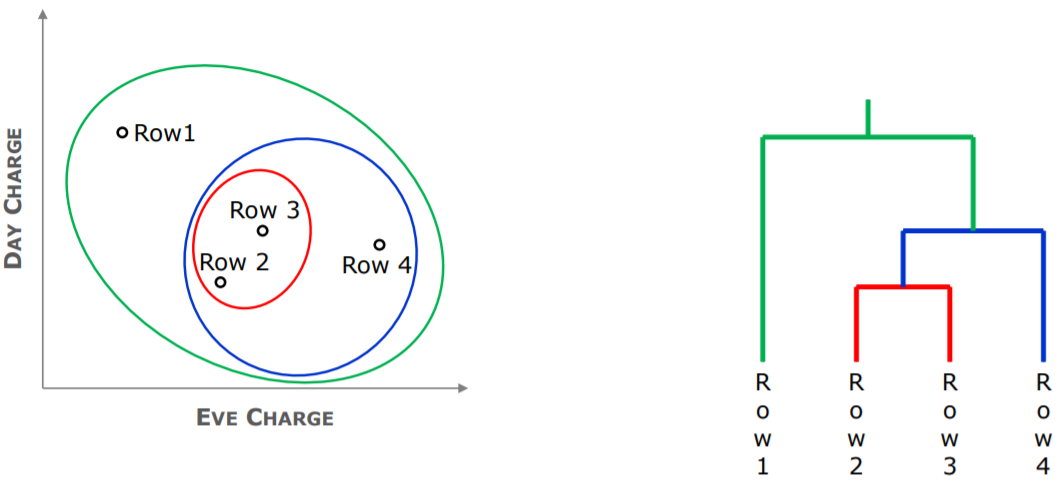
\includegraphics[height=0.45 \linewidth]{clustering/pict/cluster_aggl.png}
	\caption{da clustering gerarchico a dendrogramma}
\end{figure}

Si parte dai singoli elementi e pian piano vengono generati cluster sempre pi\`u inclusivi fino ad ottenere un unico cluster. \\

\noindent
\textbf{Passaggi}:
\begin{enumerate}
	\item Calcolare la matrice di prossimit\`a
	\item \textbf{Ripeti}
	\item Unione di due cluster vicini
	\item Aggiorna la matrice di prossimit\`a (o delle distanze) che riflette la prossimit\`a tra il nuovo cluster e il cluster originale
	\item \textbf{Finch\`e} rimane un solo cluster
\end{enumerate}
\noindent
La prossimit\`a tra cluster viene calcolata con:
\begin{itemize}
	\item  \textit{Min or Single Linkage}: minore distanza tra tutte le possibili coppie di elementi presenti nei due cluster (soluzione pi\`u ottimista)
	\item \textit{Max or Complete Linkage}: maggiore distanza tra tutte le possibili coppie di elementi presenti nei due cluster (soluzione pi\`u robusta o pessimista)
	\item \textit{Group Avarage or Avarage Linkage}: media distanza tra tutte le possibili coppie di elementi presenti nei due cluster (soluzione media - politically correct cit)
	\item \textit{metodo di Ward}: assume i cluster come rappresentati dai centroidi, misura la prossimit\`a tra due cluster come somme di scarti quadratici che risulta dalla fusione di due cluster
\end{itemize}
\noindent
\textit{Caratteristiche}:
\begin{itemize}
	\item Non risolve problemi di ottimizzazione globale
	\item pu\`o gestire cluster con dimensioni differenti, gli elementi possono anche essere pesati o meno
	\item le decisioni di unione sono definitive: non si pu\`o tornare indietro rispetto alla decisione (approccio greedy)
\end{itemize}
\noindent
\textit{Difetti}:
\begin{itemize}
	\item computazionalmente molto pesante e richiede molto spazio
	\item decisioni di unione di cluster sono subottimali quindi creano rumore
\end{itemize}

\subsection{Density-Based Clustering}
Densit\`a di regioni di oggetti che sono circondati da regioni con bassa densit\`a di oggetti.

\textbf{DBSCAN} \`e un semplice ma efficace metodo density-based. 

Vi sono diversi metodi per definire la \textit{densit\`a}, descriviamo il center-based approach: la densit\`a \`e il numero di oggetti all'interno di uno specifico raggio (\textbf{Eps}) di quell'oggetto. 

\noindent
Ci sono 3 tipi di punti:
\begin{itemize}
	\item \textbf{core point}: stanno all'interno della regione ad elevata densit\`a. \`E core pont se il numero di punti nel vicinato attorno ad esso eccede un certo \textit{threshold} MinPts, impostato dall'utente
	\item \textbf{border point} (wanna be core point): un punto che include nel suo vicinato un core point, quindi lui si considera un vicino di core point
	\item \textbf{noise point} (osservazione residuale no core o border): non \`e ne un core point ne un border point
\end{itemize}

\noindent
\textbf{Passaggi}
\begin{enumerate}
	\item Etichettare tutti i core, border, noise point
	\item Si eliminano i noise point
	\item collegano i core point che sono all'interno dei rispettivi Eps
	\item si fa ogni gruppo di core point connessi in cluster separati
	\item si assegna ciascun border point in un cluster associato ai core point pi\`u prossimo
\end{enumerate}

La scelta dei parametri \textit{MinPts} e \textit{Eps} \`e fondamentale.
\\
\\
\underline{DBSCAN vs K-medie}:
\begin{itemize}
	\item DBSCAN and K-Means assign objects to a single cluster, but K-Means assigns all
	objects while DBSCAN can discard noise objects
	\item DBSCAN can handle clusters of different sizes and shapes and it is not strongly
	affected by noise or outliers. K-means has difficulties with non-globular clusters and
	clusters of different sizes. Both algorithms perform poorly when clusters have widely
	differing densities
	\item K-Means can only be used for data that has a well defined centroid, such as mean or
	median. DBSCAN requires that its definition of density, which is based on the
	traditional Euclidean notion of density be meaningful for the data
	\item K-Means can be applied to sparse, high-dimensional data, such as document data.
	DBSCAN typically performs poorly for such data because the traditional Euclidean
	definition of density does not work well for high-dimensional data
	\item DBSCAN makes no assumption about the distribution of the data. The basic K-means
	is equivalent to a statistical clustering approach (Mixture Model) that assumes all
	clusters come from spherical Gaussian distributions with different means but the
	same covariance matrix
	\item DBSCAN and K-Means both look for clusters using all attributes, that is, they do not
	look for clusters that may involve only a sub-set of the attributes
	\item K-Means can find clusters that are not well separated, even if they overlap, but
	DBSCAN merges clusters that overlap
	\item K-Means has complexity O(m) while DBSCAN is O(m2) (except for low dimensional
	Euclidean data.)
	\item DBSCAN produces the same set of clusters from one run to another while K-Means,
	which is typically used with random initialization of centroids, does not
	\item DBSCAN automatically determines the number of clusters, for K-Means the number
	of clusters needs to be specified as a parameter
\end{itemize}
\noindent
Vi sono altri algoritmi di density-based:
\begin{itemize}
	\item Grid-based clustering
	\item subspace clustering
	\item kernel density function
\end{itemize}

\subsection{Graph-based Clustering Algorithm}
Gi\`a gli algoritmi a rappresentazione gerarchica possono essere visti come graph-based. 

Sparsificare: tagliare, rimuovere certi archi che non superano la verifica di una certa condizione (Es. tutti gli archi che non superano una certa soglia, oppure un concetto di vicinato). 

Definire una misura di similarit\`a tra due oggetti basati sul numero di nearest neighbors. 

Definire oggetti core e costruire cluster attoro ad essi. Necessita di concetti di densit\`a e prossimit\`a.

Utilizza l'informazione nel grafo di prossimit\`a per fornire una maggiore valutazione di specialit\`a in cui due cluster dovrebbero essere uniti. 

Grafo di prossimit\`a stabilisce dei pesi tra i vari nodi che \`e il costo da percorrere tra un nodo ed un altro, \`e rappresentazione della matrice delle distanze. 

I legami di similarit\`a tra nodi vengono suddivisi in \textit{sufficientemente vicini} (superano il threshold) e \textit{non vicini} quindi con vicinanza minore rispetto al threshold. Vengono quindi rimossi gli archi che non superano il threshold, questo significa \textit{sparsificare} la matrice. Viene cos\`i generato il grafo di prossimit\`a sparsificato.

Definiamo quindi il \textbf{K-Nearest Neighbor}\\
se fisso k = 3 scelgo per ogni riga della matrice delle prossimit\`a i primi 3 valori degli archi per come vicinato. 

2 modi di procedere: threshold o k neighbors.

La sparsificazione riduce anche di molto il numero di elementi del dataset. Il clustering lavora molto meglio in quanto si lavora in un concetto di vicinanza. Algoritmi su grafi partizionati possono essere usati. 

\subsection{Altri algoritmi}
Non sempre purtroppo la sparsificazione del grafo porta ad un grafo sconnesso. L'idea \`e di ciclare la sparsificazione finch\`e non otterr\`o dei grafi partizionati ben definiti. 

\textbf{Minimum spanning tree} o albero di supporto a costo minimo:
\begin{itemize}
	\item non ha cicli
	\item contiene tutti i nodi dell'albero
	\item ha il minimo costo totale dei pesi associati ai suoi alberi di tutti i possibili spanning tree
\end{itemize}
\noindent
\textbf{MST divisive hierarchical clustering Algorithm}
\begin{enumerate}
	\item Calcola il MST per grafo di dissimilarit\`a
	\item \textbf{Ripeti}
	\item Crea un nuovo cluster per rompere il collegamento corrispondente alla pi\`u grande dissimilarit\`a
	\item \textbf{Finch\`e} rimangono solo cluster singoli
\end{enumerate}
\noindent
Algoritmo \textbf{Opossum}:
\begin{enumerate}
	\item Caclola il grafo di similarit\`a sparso
	\item partiziona il grafo in k componenti distinte (cluster) usando METIS
\end{enumerate}
\noindent
Altro algoritmo \textbf{Camaleon}.

Quando si visualizza il dendrogramma, si possono visualizzare le distanze e solitamente ha una forma a "gomito" la soluzione ottimale \`e solitamente quella che precede la salita finale del comito. Un buon dendrogramma ha grandi salti prima di aggregare insieme (salti grandi significa che se raggruppo genero un errore importante quindi \`e positivo per la valutazione del clustering). 

\section{Lezione - Clustering Evaluation}

L'efficienza di un algritmo di clustering viene valutato tramite:
\begin{itemize}
	\item similarit\`a
	\item esclusivit\`a dei clustering o misure fuzzy di sovrapposizione
	\item completo o parziale clustering
\end{itemize}

Innanzitutto scelgo alcuni algoritmi candidati da voler implementare in base alla tipologia di dati che ho. L'utilit\`a di utilizzarne diversi e poterli confrontare. Bisogna impostare un'insieme di esperimenti equi per poterli valutare correttamente (stessi dati, chiare differenze di parametri ecc). 
Il problema \`e che \`e molto complesso valutare i cluster visto che non so esattamente cosa sto cercando. 

I problemi grossi nella valutazione sono:
\begin{itemize}
	\item determinare la tendenza dei cluster (che non siano fatti a caso)
	\item determinare il numero corretto di cluster (qualunque cosa significhi)
\end{itemize} 

abbiamo 3 diversi tipi di indici:
\begin{itemize}
	\item \textbf{Esterni o supervisionati}: misure che estendono i cluster scoperti con alcune strutture esterne (sapendo circa la verit\`a sul problema)
	\item \textbf{Interni o non supervisionati}: misure di similarit\`a di cluster in particolare le strutture in base a informazioni esterne, possono essere:
	\begin{itemize}
		\item Misure di coesione: determina la connessione tra elementi di un cluster
		\item misure di separazione: quanto sono ben distiniti i cluster 
	\end{itemize}
	\item \textbf{Relativi}: compara differenti clustering
\end{itemize}

\subsection{Esterni o supervisionati}
$P = \{P_1, ..., P_R\}$ partizione di un dataset di m (oggetti record) in R categorie, possono essere partizionati con algoritmi in k cluster $C= \{C_1, ..., C_K\}$.

Casi:
\begin{enumerate}
	\item (\textbf{a}) x e y appartengono allo \underline{stesso} cluster di C e alla \underline{stessa} categoria di P
	\item (\textbf{b}) x e y appartengono allo \underline{stesso} cluster di C e a \textit{differenti} categorie di P
	\item (\textbf{c}) x e y appartengono a \textit{differenti} cluster di C e alla \underline{stessa} categoria di P
	\item (\textbf{d}) x e y appartengono a \textit{differenti} cluster di C e a \textit{differenti} categorie di P
\end{enumerate}

Numero totale di coppie che si possono formare:
\[ M = \frac{m x (m-1)}{2} = a + b + c + d\]

Rand: \[R = \frac{a + d}{M}\] con $R \in [0,1]$

Jaccard: \[J = \frac{a}{a + b + c}\] con $J \in [0,1]$

Fowlkes and Mallows: \[FM = \sqrt{\frac{a}{a + b} x \frac{a}{a + c}}\]

$\Gamma$ statistics

\subsection{Interni o non supervisionati}

Molte misure di validit\`a del partizionamento dei cluster si basano sulla \textbf{coesione} e sulla \textbf{separazione}. Noi di base vogliamo un valore di coesione alto ed un valore di separazione basso.

Ci si basa sul concetto di grafo (graph-based), la coesione di un cluster pu\`o essre definita come a somma dei pesi degli archi inn un grafo di prossimit\`a che connette i punti all'interno del cluster. 

\[ cohesion(C_i) = \sum_{x, u \int C_i} proximity(x,y) = \sum_{x y \in C_i} similarity(x,y)\]

La similarit\`a \`e quindi inversamente proporzionale alla dissimilarit\`a. 
La separazione \`e valutata secondo la somma dell prossimit\`a di nodi che non appartengono allo stesso cluster.

Per i cluster prototype-based la coesione \`e valutata rispetto al centroide che ne rappresenta il prototipo; la separazione \`e misurata sulla prossimit\`a del centroide o prototipo del cluster. Altro metodo per la separazione \`e la valutazione rispetto al centroide generato dai due cluster.

La validit\`a \`e valutata in questo modo: $overall validity = \sum_{i = 1}^{K} w_i \cdot validity(C_i)$, dobbiamo decidere per\`o il peso da applicarvi ($W_i$). 


Importante capire che alle volte separare un cluster potrebbe migliorare le misure di coesione, quando ho valori di coesione bassi.

Se invece ho valori di coesione buoni ma valori di separazione alti allora provando ad unirli si raggiungono cluster pi\`u coesi. 

La valutazione che sta all'interno del cluster contribuisce maggiormente informazione alla coesione e separazione, invece per le osservazioni pi\`u esterne queste valutazioni possono non essere cos\`i utili. Pertanto \`e stato definito l'\textbf{indice di Silhouette}. questo indice combina coesione e separazione per l'i-esimo oggetto e si definisce in questo modo:

\[s_i = \frac{b_i - a_i}{max(a_i,b_i)} \in [-1,+1]\]

dove $a_i$ \`e la media della distanza tra l'oggetto i-esimo e gli altri oggetti nel cluster, $b_i$ la minima distanza media dell'oggetto i-esimo a tutti gli altri oggetti di ogni custer diverso dal cluster di partenza dell'oggetto.

(es. se $a_i = 0$ allora $s_i = 1$ perch\`e si trova nel cluster migliore. se ha invece valore $< 0$ significa che se avessi assegnato ad un altro cluster avrei avuto un indice di silhouette pi\`u alto)

L'avarage Silhouette coefficient di un cluster da un valore di silhouette medio 

Per il clustering gerarchico viene definito il Cophenetic Correlation Coefficient: 
Si considera la matrice di prossimit\`a e la matrice cophenetica.
Cophenac matrix \`e la matrice che tiene conto delle distanze tra coppie di osservazioni raggruppate all'interno di uno stesso cluster. Il valore varia da $[-1,1]$. Pi\`u il valore \`e vicino a 1 meglio l'algoritmo gerarchico fitta.

\subsection{Paradigma di validit\`a}
Rispondere alla domanda se il nostro dataset tende ad essere clusterizzabile.

Vengono considerati criteri interni ed esterni legati a metodi statistici e test di ipotesi. 

Se non ci fosse nessuna struttura dei dati (ipotesi NULLA). 

\begin{itemize}
	\item Random Position Hypothesis in tutte le location di m osservazioni in specifiche regioni n-dimensionali sono equamente buone $\rightarrow$ per ratio data
	\item Random Graph Hyothesis la matrice di prossimit\`a ha rank equamente buoni $\rightarrow$ per prossimit\`a ordinali tra coppie di osservazioni
	\item Random Level Hypothesis tutte le permutazioni delle label di m osservazioni sono equamente buone $\rightarrow$ per tutti i tipi di dati
\end{itemize}

A questo punto valuto in base alla distribuzione sotto l'ipotesi nulla e ci calcolo l'indice. Se il valore dell'indice \`e all'interno del quantile fissato ($\alpha$) posso affermare che ci sia struttura nel dataset, se invece l'ipotesi \`e rigettata allora si sa che il clustering sviluppato non ha struttura pertanto pu\`o essere mostrata al proprio interlocutore l'algoritmo sviluppato. 

\subsection{Selezione del numero di cluster}
A senso porsi questa domanda se si \`e prima rilevato che vi \`e struttura di clustering. 

I criteri \textbf{relativi} \`e un uso particolare delle misure di clsustering per comprendere il numero ottimale di cluster. Si proietta lo spazio delle osservazioni in uno spazio di dimensione minore e da questo si utilizzano delle tecniche di valutazione.

Gli indici principali sono:
\begin{itemize}
	\item Calinski and Harabasz: seleziono il numero di k che ottimizza il numero di cluster
	\item Dunn: simile a quello sopra
	\item Devies-Bouldin: minimizzo K per l'ottimo numero di cluster
\end{itemize}

Misure miste di probabilit\`a model-based clustering sono:
\begin{itemize}
	\item Akaike Information Criterion (AIC)
	\item Minimum Description Length (MDL)
	\item Bayesian Information Criterion (BIC)
\end{itemize}

Per l'algoritmo di clustering richiede un input di numero di clsuter K dagli utenti una sequenza di strutture di clustering ottenute eseguendo l'algoritmo motlre volte dove K spazia da $K_{min}$ a $K_{max}$.